% Options for packages loaded elsewhere
\PassOptionsToPackage{unicode}{hyperref}
\PassOptionsToPackage{hyphens}{url}
%
\documentclass[
]{book}
\usepackage{amsmath,amssymb}
\usepackage{lmodern}
\usepackage{iftex}
\ifPDFTeX
  \usepackage[T1]{fontenc}
  \usepackage[utf8]{inputenc}
  \usepackage{textcomp} % provide euro and other symbols
\else % if luatex or xetex
  \usepackage{unicode-math}
  \defaultfontfeatures{Scale=MatchLowercase}
  \defaultfontfeatures[\rmfamily]{Ligatures=TeX,Scale=1}
\fi
% Use upquote if available, for straight quotes in verbatim environments
\IfFileExists{upquote.sty}{\usepackage{upquote}}{}
\IfFileExists{microtype.sty}{% use microtype if available
  \usepackage[]{microtype}
  \UseMicrotypeSet[protrusion]{basicmath} % disable protrusion for tt fonts
}{}
\makeatletter
\@ifundefined{KOMAClassName}{% if non-KOMA class
  \IfFileExists{parskip.sty}{%
    \usepackage{parskip}
  }{% else
    \setlength{\parindent}{0pt}
    \setlength{\parskip}{6pt plus 2pt minus 1pt}}
}{% if KOMA class
  \KOMAoptions{parskip=half}}
\makeatother
\usepackage{xcolor}
\IfFileExists{xurl.sty}{\usepackage{xurl}}{} % add URL line breaks if available
\IfFileExists{bookmark.sty}{\usepackage{bookmark}}{\usepackage{hyperref}}
\hypersetup{
  pdftitle={gibbonR: An R package for the automated detection and classification of female gibbon calls from long-term acoustic recordings},
  pdfauthor={Dena J. Clink},
  hidelinks,
  pdfcreator={LaTeX via pandoc}}
\urlstyle{same} % disable monospaced font for URLs
\usepackage{color}
\usepackage{fancyvrb}
\newcommand{\VerbBar}{|}
\newcommand{\VERB}{\Verb[commandchars=\\\{\}]}
\DefineVerbatimEnvironment{Highlighting}{Verbatim}{commandchars=\\\{\}}
% Add ',fontsize=\small' for more characters per line
\usepackage{framed}
\definecolor{shadecolor}{RGB}{248,248,248}
\newenvironment{Shaded}{\begin{snugshade}}{\end{snugshade}}
\newcommand{\AlertTok}[1]{\textcolor[rgb]{0.94,0.16,0.16}{#1}}
\newcommand{\AnnotationTok}[1]{\textcolor[rgb]{0.56,0.35,0.01}{\textbf{\textit{#1}}}}
\newcommand{\AttributeTok}[1]{\textcolor[rgb]{0.77,0.63,0.00}{#1}}
\newcommand{\BaseNTok}[1]{\textcolor[rgb]{0.00,0.00,0.81}{#1}}
\newcommand{\BuiltInTok}[1]{#1}
\newcommand{\CharTok}[1]{\textcolor[rgb]{0.31,0.60,0.02}{#1}}
\newcommand{\CommentTok}[1]{\textcolor[rgb]{0.56,0.35,0.01}{\textit{#1}}}
\newcommand{\CommentVarTok}[1]{\textcolor[rgb]{0.56,0.35,0.01}{\textbf{\textit{#1}}}}
\newcommand{\ConstantTok}[1]{\textcolor[rgb]{0.00,0.00,0.00}{#1}}
\newcommand{\ControlFlowTok}[1]{\textcolor[rgb]{0.13,0.29,0.53}{\textbf{#1}}}
\newcommand{\DataTypeTok}[1]{\textcolor[rgb]{0.13,0.29,0.53}{#1}}
\newcommand{\DecValTok}[1]{\textcolor[rgb]{0.00,0.00,0.81}{#1}}
\newcommand{\DocumentationTok}[1]{\textcolor[rgb]{0.56,0.35,0.01}{\textbf{\textit{#1}}}}
\newcommand{\ErrorTok}[1]{\textcolor[rgb]{0.64,0.00,0.00}{\textbf{#1}}}
\newcommand{\ExtensionTok}[1]{#1}
\newcommand{\FloatTok}[1]{\textcolor[rgb]{0.00,0.00,0.81}{#1}}
\newcommand{\FunctionTok}[1]{\textcolor[rgb]{0.00,0.00,0.00}{#1}}
\newcommand{\ImportTok}[1]{#1}
\newcommand{\InformationTok}[1]{\textcolor[rgb]{0.56,0.35,0.01}{\textbf{\textit{#1}}}}
\newcommand{\KeywordTok}[1]{\textcolor[rgb]{0.13,0.29,0.53}{\textbf{#1}}}
\newcommand{\NormalTok}[1]{#1}
\newcommand{\OperatorTok}[1]{\textcolor[rgb]{0.81,0.36,0.00}{\textbf{#1}}}
\newcommand{\OtherTok}[1]{\textcolor[rgb]{0.56,0.35,0.01}{#1}}
\newcommand{\PreprocessorTok}[1]{\textcolor[rgb]{0.56,0.35,0.01}{\textit{#1}}}
\newcommand{\RegionMarkerTok}[1]{#1}
\newcommand{\SpecialCharTok}[1]{\textcolor[rgb]{0.00,0.00,0.00}{#1}}
\newcommand{\SpecialStringTok}[1]{\textcolor[rgb]{0.31,0.60,0.02}{#1}}
\newcommand{\StringTok}[1]{\textcolor[rgb]{0.31,0.60,0.02}{#1}}
\newcommand{\VariableTok}[1]{\textcolor[rgb]{0.00,0.00,0.00}{#1}}
\newcommand{\VerbatimStringTok}[1]{\textcolor[rgb]{0.31,0.60,0.02}{#1}}
\newcommand{\WarningTok}[1]{\textcolor[rgb]{0.56,0.35,0.01}{\textbf{\textit{#1}}}}
\usepackage{longtable,booktabs,array}
\usepackage{calc} % for calculating minipage widths
% Correct order of tables after \paragraph or \subparagraph
\usepackage{etoolbox}
\makeatletter
\patchcmd\longtable{\par}{\if@noskipsec\mbox{}\fi\par}{}{}
\makeatother
% Allow footnotes in longtable head/foot
\IfFileExists{footnotehyper.sty}{\usepackage{footnotehyper}}{\usepackage{footnote}}
\makesavenoteenv{longtable}
\usepackage{graphicx}
\makeatletter
\def\maxwidth{\ifdim\Gin@nat@width>\linewidth\linewidth\else\Gin@nat@width\fi}
\def\maxheight{\ifdim\Gin@nat@height>\textheight\textheight\else\Gin@nat@height\fi}
\makeatother
% Scale images if necessary, so that they will not overflow the page
% margins by default, and it is still possible to overwrite the defaults
% using explicit options in \includegraphics[width, height, ...]{}
\setkeys{Gin}{width=\maxwidth,height=\maxheight,keepaspectratio}
% Set default figure placement to htbp
\makeatletter
\def\fps@figure{htbp}
\makeatother
\setlength{\emergencystretch}{3em} % prevent overfull lines
\providecommand{\tightlist}{%
  \setlength{\itemsep}{0pt}\setlength{\parskip}{0pt}}
\setcounter{secnumdepth}{5}
\usepackage{booktabs}
\usepackage{amsthm}
\makeatletter
\def\thm@space@setup{%
  \thm@preskip=8pt plus 2pt minus 4pt
  \thm@postskip=\thm@preskip
}
\makeatother
\ifLuaTeX
  \usepackage{selnolig}  % disable illegal ligatures
\fi
\usepackage[]{natbib}
\bibliographystyle{apalike}

\title{gibbonR: An R package for the automated detection and classification of female gibbon calls from long-term acoustic recordings}
\author{Dena J. Clink}
\date{2022-10-15}

\begin{document}
\maketitle

{
\setcounter{tocdepth}{1}
\tableofcontents
}
\hypertarget{getting-started}{%
\chapter{Getting started}\label{getting-started}}

\hypertarget{you-can-install-the-development-version-from-github-with}{%
\section{\texorpdfstring{You can install the development version from \href{https://github.com/DenaJGibbon}{GitHub} with:}{You can install the development version from GitHub with:}}\label{you-can-install-the-development-version-from-github-with}}

\begin{Shaded}
\begin{Highlighting}[]
\CommentTok{\# install.packages("devtools")}
\CommentTok{\# devtools::install\_github("DenaJGibbon/gibbonR")}

\FunctionTok{library}\NormalTok{(gibbonR)}
\CommentTok{\#\textgreater{} Loading required package: stringr}
\CommentTok{\#\textgreater{} Loading required package: e1071}
\CommentTok{\#\textgreater{} Loading required package: randomForest}
\CommentTok{\#\textgreater{} randomForest 4.7{-}1}
\CommentTok{\#\textgreater{} Type rfNews() to see new features/changes/bug fixes.}
\CommentTok{\#\textgreater{} Loading required package: tuneR}
\CommentTok{\#\textgreater{} Loading required package: seewave}
\end{Highlighting}
\end{Shaded}

\hypertarget{part-1.-prepare-training-data}{%
\chapter{Part 1. Prepare Training Data}\label{part-1.-prepare-training-data}}

In `gibbonR' there are two ways that you can format your training data. The first can be a set of labelled .wav clips with the class indicated in the name of the file (e.g., `gibbon\_01.wav' and `noise\_01.wav'). The second is to have a folder of selection tables created in Raven Pro (K. Lisa Yang Center for Conservation Bioacoustics) and a folder with the associated `.wav' files. For the second approach there must be an annotation column indicating the call type and it is assumed that all signals of interest are annotated, and the rest of the files contain only background noise.

\hypertarget{part-1a.-training-data-with-labeled-.wav-clips}{%
\section{Part 1A. Training Data with Labeled .wav clips}\label{part-1a.-training-data-with-labeled-.wav-clips}}

\hypertarget{read-in-clips-and-calculate-mfccs}{%
\subsection{Read in clips and calculate MFCCs}\label{read-in-clips-and-calculate-mfccs}}

\begin{Shaded}
\begin{Highlighting}[]
\NormalTok{TrainingWavFilesDir }\OtherTok{\textless{}{-}} 
  \StringTok{"/Users/denaclink/Desktop/RStudio Projects/gibbonR/data/MultipleSoundClasses/"}

\NormalTok{trainingdata }\OtherTok{\textless{}{-}}\NormalTok{ gibbonR}\SpecialCharTok{::}\FunctionTok{MFCCFunction}\NormalTok{(}\AttributeTok{input.dir=}\NormalTok{TrainingWavFilesDir, }\AttributeTok{min.freq =} \DecValTok{400}\NormalTok{, }\AttributeTok{max.freq =} \DecValTok{1600}\NormalTok{,}\AttributeTok{win.avg=}\StringTok{"TRUE"}\NormalTok{)}


\NormalTok{trainingdata}\SpecialCharTok{$}\NormalTok{class }\OtherTok{\textless{}{-}} \FunctionTok{as.factor}\NormalTok{(trainingdata}\SpecialCharTok{$}\NormalTok{class)}
\end{Highlighting}
\end{Shaded}

\hypertarget{compare-random-forest-and-support-vector-machine-for-supervised-classification}{%
\subsection{Compare Random Forest and Support Vector Machine for Supervised Classification}\label{compare-random-forest-and-support-vector-machine-for-supervised-classification}}

\begin{Shaded}
\begin{Highlighting}[]

\NormalTok{trainingdata}\SpecialCharTok{$}\NormalTok{class }\OtherTok{\textless{}{-}} \FunctionTok{as.factor}\NormalTok{(trainingdata}\SpecialCharTok{$}\NormalTok{class)}


\NormalTok{ml.model.svm }\OtherTok{\textless{}{-}}\NormalTok{ e1071}\SpecialCharTok{::}\FunctionTok{svm}\NormalTok{(trainingdata[, }\DecValTok{2}\SpecialCharTok{:}\FunctionTok{ncol}\NormalTok{(trainingdata)], trainingdata}\SpecialCharTok{$}\NormalTok{class, }\AttributeTok{kernel =} \StringTok{"radial"}\NormalTok{, }
                           \AttributeTok{cross =} \DecValTok{25}\NormalTok{,}
                           \AttributeTok{probability =} \ConstantTok{TRUE}\NormalTok{)}

\FunctionTok{print}\NormalTok{(}\FunctionTok{paste}\NormalTok{(}\StringTok{\textquotesingle{}SVM accuracy\textquotesingle{}}\NormalTok{,ml.model.svm}\SpecialCharTok{$}\NormalTok{tot.accuracy))}
\CommentTok{\#\textgreater{} [1] "SVM accuracy 88"}


\NormalTok{ml.model.rf }\OtherTok{\textless{}{-}}\NormalTok{ randomForest}\SpecialCharTok{::}\FunctionTok{randomForest}\NormalTok{(}\AttributeTok{x=}\NormalTok{trainingdata[, }\DecValTok{2}\SpecialCharTok{:}\FunctionTok{ncol}\NormalTok{(trainingdata)], }\AttributeTok{y =}\NormalTok{ trainingdata}\SpecialCharTok{$}\NormalTok{class)}


\FunctionTok{print}\NormalTok{(ml.model.rf)}
\CommentTok{\#\textgreater{} }
\CommentTok{\#\textgreater{} Call:}
\CommentTok{\#\textgreater{}  randomForest(x = trainingdata[, 2:ncol(trainingdata)], y = trainingdata$class) }
\CommentTok{\#\textgreater{}                Type of random forest: classification}
\CommentTok{\#\textgreater{}                      Number of trees: 500}
\CommentTok{\#\textgreater{} No. of variables tried at each split: 13}
\CommentTok{\#\textgreater{} }
\CommentTok{\#\textgreater{}         OOB estimate of  error rate: 9.33\%}
\CommentTok{\#\textgreater{} Confusion matrix:}
\CommentTok{\#\textgreater{}               female.gibbon leaf.monkey noise solo.gibbon class.error}
\CommentTok{\#\textgreater{} female.gibbon            19           0     1           0        0.05}
\CommentTok{\#\textgreater{} leaf.monkey               0          12     3           0        0.20}
\CommentTok{\#\textgreater{} noise                     0           1    18           1        0.10}
\CommentTok{\#\textgreater{} solo.gibbon               0           0     1          19        0.05}
\end{Highlighting}
\end{Shaded}

\hypertarget{part-1b.-training-data-with-raven-selection-tables}{%
\section{Part 1B. Training Data with Raven Selection Tables}\label{part-1b.-training-data-with-raven-selection-tables}}

\hypertarget{prepare-training-data-from-labeled-annotations}{%
\subsection{Prepare training data from labeled annotations}\label{prepare-training-data-from-labeled-annotations}}

\begin{Shaded}
\begin{Highlighting}[]
\CommentTok{\# Specify the folder where the training data will be saved}
\NormalTok{TrainingDataFolderLocation }\OtherTok{\textless{}{-}} \StringTok{"/Users/denaclink/Desktop/RStudio Projects/gibbonR/data/TrainingDataFromRavenSelectionTables"}

\CommentTok{\# Directory with annotated selection tables}
\NormalTok{AnnotatedSelectionTables }\OtherTok{\textless{}{-}} \FunctionTok{list.files}\NormalTok{(}\StringTok{"/Users/denaclink/Desktop/RStudio Projects/gibbonR/data/SelectionTables/GibbonTrainingSelectionTables/"}\NormalTok{,}
                                       \AttributeTok{full.names =}\NormalTok{ T)}

\CommentTok{\# Directory with corresponding .wav files}
\NormalTok{AnnotatedWaveFiles }\OtherTok{\textless{}{-}} \FunctionTok{list.files}\NormalTok{(}\StringTok{"/Users/denaclink/Library/CloudStorage/Box{-}Box/gibbonRSampleFiles/GibbonTrainingFiles/"}\NormalTok{,}\AttributeTok{full.names =}\NormalTok{ T)}
\NormalTok{AnnotatedWaveFilesShort }\OtherTok{\textless{}{-}} \FunctionTok{list.files}\NormalTok{(}\StringTok{"/Users/denaclink/Library/CloudStorage/Box{-}Box/gibbonRSampleFiles/GibbonTrainingFiles/"}\NormalTok{,}\AttributeTok{full.names =}\NormalTok{ F)}
\NormalTok{AnnotatedWaveFilesShort }\OtherTok{\textless{}{-}} \FunctionTok{str\_split\_fixed}\NormalTok{(AnnotatedWaveFilesShort,}\AttributeTok{pattern =} \StringTok{\textquotesingle{}.wav\textquotesingle{}}\NormalTok{, }\AttributeTok{n=}\DecValTok{2}\NormalTok{)[,}\DecValTok{1}\NormalTok{]}

\CommentTok{\# Loop to cut out the corresponding annotations into short clips}
\ControlFlowTok{for}\NormalTok{(i }\ControlFlowTok{in} \DecValTok{1}\SpecialCharTok{:} \FunctionTok{length}\NormalTok{(AnnotatedSelectionTables))\{}
  
  \CommentTok{\# Read in selection table}
\NormalTok{  TempSelectionTable }\OtherTok{\textless{}{-}} \FunctionTok{read.delim2}\NormalTok{(AnnotatedSelectionTables[i])}
  
  \CommentTok{\# Find the corresponding soundfile}
\NormalTok{  SoundFileIndex }\OtherTok{\textless{}{-}} \FunctionTok{which}\NormalTok{(}\FunctionTok{str\_detect}\NormalTok{(AnnotatedSelectionTables[i],AnnotatedWaveFilesShort))}
  
\NormalTok{  TempAnnotateWave }\OtherTok{\textless{}{-}} \FunctionTok{readWave}\NormalTok{(AnnotatedWaveFiles[SoundFileIndex])}
  
\NormalTok{  ShortSoundClips }\OtherTok{\textless{}{-}} \FunctionTok{lapply}\NormalTok{(}\DecValTok{1}\SpecialCharTok{:}\FunctionTok{nrow}\NormalTok{(TempSelectionTable),}
                                \ControlFlowTok{function}\NormalTok{(j) }\FunctionTok{extractWave}\NormalTok{(TempAnnotateWave,}
                                                        \AttributeTok{from=} \FunctionTok{as.numeric}\NormalTok{(TempSelectionTable[j,]}\SpecialCharTok{$}\NormalTok{Begin.Time..s.),}
                                                        \AttributeTok{to=}\FunctionTok{as.numeric}\NormalTok{(TempSelectionTable[j,]}\SpecialCharTok{$}\NormalTok{ End.Time..s.),}
                                                        \AttributeTok{xunit =} \FunctionTok{c}\NormalTok{(}\StringTok{"time"}\NormalTok{),}\AttributeTok{plot=}\NormalTok{F,}\AttributeTok{output=}\StringTok{"Wave"}\NormalTok{))}
  \CommentTok{\# Write wave files to folder}
  \ControlFlowTok{for}\NormalTok{(k }\ControlFlowTok{in} \DecValTok{1}\SpecialCharTok{:}\FunctionTok{length}\NormalTok{(ShortSoundClips))\{}
\NormalTok{    TempClip }\OtherTok{\textless{}{-}}\NormalTok{ ShortSoundClips[[k]]}
\NormalTok{    WavFileName }\OtherTok{\textless{}{-}} \FunctionTok{paste}\NormalTok{(TrainingDataFolderLocation,}\StringTok{\textquotesingle{}/female.gibbon\_\textquotesingle{}}\NormalTok{, k, }\StringTok{\textquotesingle{}.wav\textquotesingle{}}\NormalTok{,}\AttributeTok{sep=}\StringTok{""}\NormalTok{)}
    \FunctionTok{writeWave}\NormalTok{(TempClip,WavFileName,}\AttributeTok{extensible =}\NormalTok{ F)}
\NormalTok{  \}}
  
  
\NormalTok{\}}
\end{Highlighting}
\end{Shaded}

\hypertarget{prepare-noise-training-data-from-files-without-target-signal}{%
\subsection{Prepare noise training data from files without target signal}\label{prepare-noise-training-data-from-files-without-target-signal}}

\begin{Shaded}
\begin{Highlighting}[]
\CommentTok{\# Specify the folder where the training data will be saved}
\NormalTok{TrainingDataFolderLocation }\OtherTok{\textless{}{-}} \StringTok{"/Users/denaclink/Desktop/RStudio Projects/gibbonR/data/TrainingDataFromRavenSelectionTables/"}

\CommentTok{\# Directory with annotated selection tables}
\NormalTok{NoiseSelectionTables }\OtherTok{\textless{}{-}} \FunctionTok{list.files}\NormalTok{(}\StringTok{"/Users/denaclink/Desktop/RStudio Projects/gibbonR/data/SelectionTables/NoiseSelectionTables/"}\NormalTok{,}
                                       \AttributeTok{full.names =}\NormalTok{ T)}

\CommentTok{\# Directory with corresponding .wav files}
\NormalTok{NoiseWaveFiles }\OtherTok{\textless{}{-}} \FunctionTok{list.files}\NormalTok{(}\StringTok{"/Users/denaclink/Library/CloudStorage/Box{-}Box/gibbonRSampleFiles/NoiseFiles/"}\NormalTok{,}\AttributeTok{full.names =}\NormalTok{ T)}
\NormalTok{NoiseWaveFilesShort }\OtherTok{\textless{}{-}} \FunctionTok{list.files}\NormalTok{(}\StringTok{"/Users/denaclink/Library/CloudStorage/Box{-}Box/gibbonRSampleFiles/NoiseFiles/"}\NormalTok{,}\AttributeTok{full.names =}\NormalTok{ F)}
\NormalTok{NoiseWaveFilesShort }\OtherTok{\textless{}{-}} \FunctionTok{str\_split\_fixed}\NormalTok{(NoiseWaveFilesShort,}\AttributeTok{pattern =} \StringTok{\textquotesingle{}.wav\textquotesingle{}}\NormalTok{, }\AttributeTok{n=}\DecValTok{2}\NormalTok{)[,}\DecValTok{1}\NormalTok{]}

\ControlFlowTok{for}\NormalTok{(i }\ControlFlowTok{in} \DecValTok{1}\SpecialCharTok{:}\FunctionTok{length}\NormalTok{(NoiseSelectionTables))\{}
  
  \CommentTok{\# Find the corresponding soundfile}
\NormalTok{  SoundFileIndex }\OtherTok{\textless{}{-}} \FunctionTok{which}\NormalTok{(}\FunctionTok{str\_detect}\NormalTok{(NoiseSelectionTables[i],NoiseWaveFilesShort))}

  \FunctionTok{DetectBLED}\NormalTok{(}\AttributeTok{input=}\NormalTok{NoiseWaveFiles[SoundFileIndex],}
           \AttributeTok{min.freq =} \DecValTok{400}\NormalTok{, }
           \AttributeTok{max.freq =} \DecValTok{1600}\NormalTok{,}
           \AttributeTok{noise.quantile.val=}\FloatTok{0.3}\NormalTok{,}
           \AttributeTok{file.type=}\StringTok{\textquotesingle{}wav\textquotesingle{}}\NormalTok{,}
           \AttributeTok{spectrogram.window =}\DecValTok{512}\NormalTok{,}
           \AttributeTok{pattern.split =} \StringTok{".wav"}\NormalTok{, }
           \AttributeTok{min.signal.dur =} \DecValTok{3}\NormalTok{,}
           \AttributeTok{max.sound.event.dur =} \DecValTok{12}\NormalTok{, }
           \AttributeTok{output =} \StringTok{"wav"}\NormalTok{,}
           \AttributeTok{wav.output =} \StringTok{"TRUE"}\NormalTok{, }
           \AttributeTok{output.dir =}\NormalTok{ TrainingDataFolderLocation,}
           \AttributeTok{swift.time=}\ConstantTok{TRUE}\NormalTok{,}
           \AttributeTok{time.start=}\DecValTok{06}\NormalTok{,}
           \AttributeTok{time.stop=}\DecValTok{11}\NormalTok{,}
           \AttributeTok{write.csv.output=}\ConstantTok{TRUE}\NormalTok{,}
           \AttributeTok{verbose=}\ConstantTok{TRUE}\NormalTok{,}
           \AttributeTok{random.sample=}\ConstantTok{FALSE}\NormalTok{)}
\NormalTok{\}}
\end{Highlighting}
\end{Shaded}

\hypertarget{now-read-in-clips-based-on-raven-selection-tables-and-calculate-mfccs}{%
\subsection{Now read in clips based on Raven Selection tables and calculate MFCCs}\label{now-read-in-clips-based-on-raven-selection-tables-and-calculate-mfccs}}

\begin{Shaded}
\begin{Highlighting}[]

\NormalTok{TrainingWavFilesDir }\OtherTok{\textless{}{-}} 
  \StringTok{"/Users/denaclink/Desktop/RStudio Projects/gibbonR/data/TrainingDataFromRavenSelectionTables/"}

\NormalTok{trainingdata }\OtherTok{\textless{}{-}}\NormalTok{ gibbonR}\SpecialCharTok{::}\FunctionTok{MFCCFunction}\NormalTok{(}\AttributeTok{input.dir=}\NormalTok{TrainingWavFilesDir, }\AttributeTok{min.freq =} \DecValTok{400}\NormalTok{, }\AttributeTok{max.freq =} \DecValTok{1600}\NormalTok{,}\AttributeTok{win.avg=}\StringTok{"TRUE"}\NormalTok{)}


\NormalTok{trainingdata}\SpecialCharTok{$}\NormalTok{class }\OtherTok{\textless{}{-}} \FunctionTok{as.factor}\NormalTok{(trainingdata}\SpecialCharTok{$}\NormalTok{class)}
\end{Highlighting}
\end{Shaded}

\hypertarget{compare-random-forest-and-support-vector-machine-for-supervised-classification-1}{%
\subsection{Compare Random Forest and Support Vector Machine for Supervised Classification}\label{compare-random-forest-and-support-vector-machine-for-supervised-classification-1}}

\begin{Shaded}
\begin{Highlighting}[]

\NormalTok{trainingdata}\SpecialCharTok{$}\NormalTok{class }\OtherTok{\textless{}{-}} \FunctionTok{as.factor}\NormalTok{(trainingdata}\SpecialCharTok{$}\NormalTok{class)}


\NormalTok{ml.model.svm }\OtherTok{\textless{}{-}}\NormalTok{ e1071}\SpecialCharTok{::}\FunctionTok{svm}\NormalTok{(trainingdata[, }\DecValTok{2}\SpecialCharTok{:}\FunctionTok{ncol}\NormalTok{(trainingdata)], trainingdata}\SpecialCharTok{$}\NormalTok{class, }\AttributeTok{kernel =} \StringTok{"radial"}\NormalTok{, }
                           \AttributeTok{cross =} \DecValTok{25}\NormalTok{,}
                           \AttributeTok{probability =} \ConstantTok{TRUE}\NormalTok{)}

\FunctionTok{print}\NormalTok{(}\FunctionTok{paste}\NormalTok{(}\StringTok{\textquotesingle{}SVM accuracy\textquotesingle{}}\NormalTok{,ml.model.svm}\SpecialCharTok{$}\NormalTok{tot.accuracy))}
\CommentTok{\#\textgreater{} [1] "SVM accuracy 98.1132075471698"}


\NormalTok{ml.model.rf }\OtherTok{\textless{}{-}}\NormalTok{ randomForest}\SpecialCharTok{::}\FunctionTok{randomForest}\NormalTok{(}\AttributeTok{x=}\NormalTok{trainingdata[, }\DecValTok{2}\SpecialCharTok{:}\FunctionTok{ncol}\NormalTok{(trainingdata)], }\AttributeTok{y =}\NormalTok{ trainingdata}\SpecialCharTok{$}\NormalTok{class)}


\FunctionTok{print}\NormalTok{(ml.model.rf)}
\CommentTok{\#\textgreater{} }
\CommentTok{\#\textgreater{} Call:}
\CommentTok{\#\textgreater{}  randomForest(x = trainingdata[, 2:ncol(trainingdata)], y = trainingdata$class) }
\CommentTok{\#\textgreater{}                Type of random forest: classification}
\CommentTok{\#\textgreater{}                      Number of trees: 500}
\CommentTok{\#\textgreater{} No. of variables tried at each split: 13}
\CommentTok{\#\textgreater{} }
\CommentTok{\#\textgreater{}         OOB estimate of  error rate: 5.66\%}
\CommentTok{\#\textgreater{} Confusion matrix:}
\CommentTok{\#\textgreater{}               female.gibbon noise class.error}
\CommentTok{\#\textgreater{} female.gibbon            24     2  0.07692308}
\CommentTok{\#\textgreater{} noise                     1    26  0.03703704}
\end{Highlighting}
\end{Shaded}

\hypertarget{part-2.-run-the-detectorclassifier}{%
\chapter{Part 2. Run the detector/classifier}\label{part-2.-run-the-detectorclassifier}}

\hypertarget{part-2a.-feature-extraction}{%
\section{Part 2a. Feature extraction}\label{part-2a.-feature-extraction}}

\begin{Shaded}
\begin{Highlighting}[]
\CommentTok{\# Specify the folder where the training data will be saved}
\NormalTok{TrainingDataFolderLocation }\OtherTok{\textless{}{-}} \StringTok{"/Users/denaclink/Desktop/RStudio Projects/gibbonR/data/TrainingDataFromRavenSelectionTables/"}
  
\NormalTok{TrainingDataMFCC }\OtherTok{\textless{}{-}} \FunctionTok{MFCCFunction}\NormalTok{(}\AttributeTok{input.dir=}\NormalTok{ TrainingDataFolderLocation, }\AttributeTok{min.freq =} \DecValTok{400}\NormalTok{, }\AttributeTok{max.freq =} \DecValTok{1600}\NormalTok{,}\AttributeTok{win.avg=}\StringTok{"TRUE"}\NormalTok{)}
  
\NormalTok{  TrainingDataMFCC}\SpecialCharTok{$}\NormalTok{class }\OtherTok{\textless{}{-}} \FunctionTok{as.factor}\NormalTok{(TrainingDataMFCC}\SpecialCharTok{$}\NormalTok{class)}
\end{Highlighting}
\end{Shaded}

\hypertarget{part-2b.-run-detectclassify}{%
\section{Part 2b. Run DetectClassify}\label{part-2b.-run-detectclassify}}

\begin{Shaded}
\begin{Highlighting}[]

\NormalTok{  TestFileDirectory }\OtherTok{\textless{}{-}} \StringTok{\textquotesingle{}/Users/denaclink/Library/CloudStorage/Box{-}Box/gibbonRSampleFiles/GibbonTestFiles\textquotesingle{}}
  
\NormalTok{  OutputDirectory }\OtherTok{\textless{}{-}}  \StringTok{"/Users/denaclink/Desktop/RStudio Projects/gibbonR/data/DetectAndClassifyOutput"}
  
  \FunctionTok{DetectAndClassify}\NormalTok{(}\AttributeTok{input=}\NormalTok{TestFileDirectory,}
                    \AttributeTok{input.type=}\StringTok{\textquotesingle{}directory\textquotesingle{}}\NormalTok{,}
                    \AttributeTok{feature.df=}\NormalTok{TrainingDataMFCC,}
                    \AttributeTok{model.type.list=}\FunctionTok{c}\NormalTok{(}\StringTok{\textquotesingle{}SVM\textquotesingle{}}\NormalTok{,}\StringTok{\textquotesingle{}RF\textquotesingle{}}\NormalTok{),}
                    \AttributeTok{tune =} \ConstantTok{TRUE}\NormalTok{,}
                    \AttributeTok{short.wav.duration=}\DecValTok{300}\NormalTok{,}
                    \AttributeTok{target.signal =} \FunctionTok{c}\NormalTok{(}\StringTok{"female.gibbon"}\NormalTok{),}
                    \AttributeTok{min.freq =} \DecValTok{400}\NormalTok{, }\AttributeTok{max.freq =} \DecValTok{1600}\NormalTok{,}
                    \AttributeTok{noise.quantile.val=}\FloatTok{0.15}\NormalTok{,}
                    \AttributeTok{time.window.number =}\DecValTok{3}\NormalTok{,}
                    \AttributeTok{n.windows =} \DecValTok{9}\NormalTok{, }\AttributeTok{num.cep =} \DecValTok{12}\NormalTok{,}
                    \AttributeTok{spectrogram.window =}\DecValTok{160}\NormalTok{,}
                    \AttributeTok{pattern.split =} \StringTok{".wav"}\NormalTok{,}
                    \AttributeTok{min.signal.dur =} \DecValTok{3}\NormalTok{,}
                    \AttributeTok{max.sound.event.dur =} \DecValTok{25}\NormalTok{,}
                    \AttributeTok{maximum.separation =}\DecValTok{1}\NormalTok{,}
                    \AttributeTok{probability.thresh.svm =} \FloatTok{0.15}\NormalTok{,}
                    \AttributeTok{probability.thresh.rf =} \FloatTok{0.15}\NormalTok{,}
                    \AttributeTok{wav.output =} \StringTok{"TRUE"}\NormalTok{,}
                    \AttributeTok{output.dir =}\NormalTok{OutputDirectory,}
                    \AttributeTok{swift.time=}\ConstantTok{TRUE}\NormalTok{,}\AttributeTok{time.start=}\DecValTok{5}\NormalTok{,}\AttributeTok{time.stop=}\DecValTok{10}\NormalTok{,}
                    \AttributeTok{write.csv.output=}\ConstantTok{FALSE}\NormalTok{,}\AttributeTok{verbose=}\ConstantTok{TRUE}\NormalTok{,}
                    \AttributeTok{random.sample=}\StringTok{\textquotesingle{}NA\textquotesingle{}}\NormalTok{)}
\CommentTok{\#\textgreater{} [1] "Machine learning in progress..."}
\CommentTok{\#\textgreater{} [1] "SVM in progress..."}
\CommentTok{\#\textgreater{} [1] "SVM accuracy 98.1132075471698"}
\CommentTok{\#\textgreater{} Time difference of 1.573478 secs}
\CommentTok{\#\textgreater{} [1] "RF in progress..."}
\CommentTok{\#\textgreater{} }
\CommentTok{\#\textgreater{} Call:}
\CommentTok{\#\textgreater{}  randomForest(x = feature.df[, 2:ncol(feature.df)], y = feature.df$class) }
\CommentTok{\#\textgreater{}                Type of random forest: classification}
\CommentTok{\#\textgreater{}                      Number of trees: 500}
\CommentTok{\#\textgreater{} No. of variables tried at each split: 13}
\CommentTok{\#\textgreater{} }
\CommentTok{\#\textgreater{}         OOB estimate of  error rate: 5.66\%}
\CommentTok{\#\textgreater{} Confusion matrix:}
\CommentTok{\#\textgreater{}               female.gibbon noise class.error}
\CommentTok{\#\textgreater{} female.gibbon            24     2  0.07692308}
\CommentTok{\#\textgreater{} noise                     1    26  0.03703704}
\CommentTok{\#\textgreater{} Time difference of 0.06214285 secs}
\CommentTok{\#\textgreater{} [1] "Classifying for target signal female.gibbon"}
\CommentTok{\#\textgreater{} [1] "Computing spectrogram for file S11\_20180217\_080003 1 out of 1"}
\CommentTok{\#\textgreater{} [1] "Running detector over sound files"}
\CommentTok{\#\textgreater{} [1] "Creating datasheet"}
\CommentTok{\#\textgreater{} [1] "System processed 7201 seconds in 14 seconds this translates to 507.4 hours processed in 1 hour"}
\end{Highlighting}
\end{Shaded}

\hypertarget{part-3.-calculate-performance-metrics}{%
\chapter{Part 3. Calculate performance metrics}\label{part-3.-calculate-performance-metrics}}

\hypertarget{part-3a.-prepare-data-for-performance-metrics}{%
\section{Part 3a. Prepare data for performance metrics}\label{part-3a.-prepare-data-for-performance-metrics}}

\begin{Shaded}
\begin{Highlighting}[]
\CommentTok{\# Set location of test file selection tables}
\NormalTok{input.dir.text.files }\OtherTok{\textless{}{-}} \StringTok{"/Users/denaclink/Desktop/RStudio Projects/gibbonR/data/SelectionTables/GibbonTestSelectionTables"}

\NormalTok{Annotatedfiles }\OtherTok{\textless{}{-}} \FunctionTok{list.files}\NormalTok{(input.dir.text.files,}\AttributeTok{full.names =}\NormalTok{ T)}

\NormalTok{ListOfAnnotatedFilesShort }\OtherTok{\textless{}{-}} \FunctionTok{list.files}\NormalTok{(input.dir.text.files,}\AttributeTok{full.names =}\NormalTok{ F)}

\NormalTok{nslash }\OtherTok{\textless{}{-}} \FunctionTok{str\_count}\NormalTok{(Annotatedfiles,}\AttributeTok{pattern =} \StringTok{\textquotesingle{}/\textquotesingle{}}\NormalTok{)[}\DecValTok{1}\NormalTok{]}\SpecialCharTok{+}\DecValTok{1}
\NormalTok{snames }\OtherTok{\textless{}{-}} \FunctionTok{str\_split\_fixed}\NormalTok{(Annotatedfiles,}\AttributeTok{pattern =} \StringTok{\textquotesingle{}/\textquotesingle{}}\NormalTok{,}\AttributeTok{n=}\NormalTok{nslash)[,nslash]}

\NormalTok{all.detections }\OtherTok{\textless{}{-}} \FunctionTok{data.frame}\NormalTok{()}
\ControlFlowTok{for}\NormalTok{(x }\ControlFlowTok{in} \DecValTok{1}\SpecialCharTok{:}\FunctionTok{length}\NormalTok{(Annotatedfiles))\{}
\NormalTok{  temp.table }\OtherTok{\textless{}{-}} \FunctionTok{read.delim2}\NormalTok{(Annotatedfiles[x],}\AttributeTok{fill =}\NormalTok{ T,}\AttributeTok{header =}\NormalTok{T)}
\NormalTok{  file.name }\OtherTok{\textless{}{-}} \FunctionTok{str\_split\_fixed}\NormalTok{(snames[x],}\AttributeTok{pattern =} \StringTok{\textquotesingle{}[.]\textquotesingle{}}\NormalTok{,}\AttributeTok{n=}\DecValTok{2}\NormalTok{)[,}\DecValTok{1}\NormalTok{]}
\NormalTok{  recorder }\OtherTok{\textless{}{-}} \FunctionTok{str\_split\_fixed}\NormalTok{(file.name,}\AttributeTok{pattern=}\StringTok{\textquotesingle{}\_\textquotesingle{}}\NormalTok{,}\AttributeTok{n=}\DecValTok{3}\NormalTok{)[,}\DecValTok{1}\NormalTok{]}
\NormalTok{  date }\OtherTok{\textless{}{-}} \FunctionTok{str\_split\_fixed}\NormalTok{(file.name,}\AttributeTok{pattern=}\StringTok{\textquotesingle{}\_\textquotesingle{}}\NormalTok{,}\AttributeTok{n=}\DecValTok{3}\NormalTok{)[,}\DecValTok{2}\NormalTok{]}
\NormalTok{  time }\OtherTok{\textless{}{-}} \FunctionTok{str\_split\_fixed}\NormalTok{(file.name,}\AttributeTok{pattern=}\StringTok{\textquotesingle{}\_\textquotesingle{}}\NormalTok{,}\AttributeTok{n=}\DecValTok{3}\NormalTok{)[,}\DecValTok{3}\NormalTok{]}
  
  \ControlFlowTok{if}\NormalTok{(}\FunctionTok{nrow}\NormalTok{(temp.table }\SpecialCharTok{\textgreater{}}\DecValTok{0}\NormalTok{))\{}
\NormalTok{    temp.table.updated }\OtherTok{\textless{}{-}} \FunctionTok{cbind.data.frame}\NormalTok{(file.name,recorder,date,time,temp.table)}
\NormalTok{  \} }\ControlFlowTok{else}\NormalTok{ \{}
\NormalTok{    temp.row }\OtherTok{\textless{}{-}} \FunctionTok{as.data.frame}\NormalTok{(}\FunctionTok{t}\NormalTok{(}\FunctionTok{rep}\NormalTok{(}\StringTok{\textquotesingle{}NA\textquotesingle{}}\NormalTok{,}\FunctionTok{ncol}\NormalTok{(temp.table))))}
    \FunctionTok{colnames}\NormalTok{(temp.row) }\OtherTok{\textless{}{-}} \FunctionTok{colnames}\NormalTok{(temp.table)}
\NormalTok{    temp.table.updated }\OtherTok{\textless{}{-}} \FunctionTok{cbind.data.frame}\NormalTok{(file.name,recorder,date,time,temp.row)}
    
\NormalTok{  \}}
\NormalTok{  all.detections }\OtherTok{\textless{}{-}} \FunctionTok{rbind.data.frame}\NormalTok{(all.detections,temp.table.updated)}
\NormalTok{\}}
\end{Highlighting}
\end{Shaded}

\hypertarget{part-3b.-identify-true-and-false-positives}{%
\section{Part 3b. Identify true and false positives}\label{part-3b.-identify-true-and-false-positives}}

\begin{Shaded}
\begin{Highlighting}[]
\NormalTok{  OutputDirectory }\OtherTok{\textless{}{-}}  \StringTok{"/Users/denaclink/Desktop/RStudio Projects/gibbonR/data/DetectAndClassifyOutput"}
    
\NormalTok{  all.combinedprecision.recall.randomiter }\OtherTok{\textless{}{-}} \FunctionTok{data.frame}\NormalTok{()}
\NormalTok{  range.secs.start }\OtherTok{\textless{}{-}} \DecValTok{6}
\NormalTok{  range.secs.end }\OtherTok{\textless{}{-}} \DecValTok{6}
  
  \DocumentationTok{\#\#\# Detections using band{-}limited energy summation}
\NormalTok{  gibbondetects }\OtherTok{\textless{}{-}}\NormalTok{ OutputDirectory}
\NormalTok{  list.ml }\OtherTok{\textless{}{-}}  \FunctionTok{list.files}\NormalTok{(gibbondetects, }\AttributeTok{full.names =}\NormalTok{ T, }\AttributeTok{pattern=}\StringTok{\textquotesingle{}.wav\textquotesingle{}}\NormalTok{)}

  
  \CommentTok{\# Need to focus on gibbons for this validation}
\NormalTok{  nslash }\OtherTok{\textless{}{-}} \FunctionTok{str\_count}\NormalTok{(list.ml[[}\DecValTok{1}\NormalTok{]],}\StringTok{\textquotesingle{}/\textquotesingle{}}\NormalTok{)}\SpecialCharTok{+}\DecValTok{1}
\NormalTok{  list.ml.signals }\OtherTok{\textless{}{-}} \FunctionTok{str\_split\_fixed}\NormalTok{(list.ml,}\AttributeTok{pattern =} \StringTok{\textquotesingle{}/\textquotesingle{}}\NormalTok{,}\AttributeTok{n=}\NormalTok{nslash)[,nslash]}
  
\NormalTok{  list.ml.signals }\OtherTok{\textless{}{-}} \FunctionTok{str\_split\_fixed}\NormalTok{(list.ml.signals,}\AttributeTok{pattern =} \StringTok{\textquotesingle{}\_\textquotesingle{}}\NormalTok{,}\AttributeTok{n=}\DecValTok{5}\NormalTok{)[,}\DecValTok{4}\NormalTok{]}
  
  
\NormalTok{  list.ml }\OtherTok{\textless{}{-}} 
\NormalTok{    list.ml[}\FunctionTok{which}\NormalTok{(list.ml.signals}\SpecialCharTok{==}\StringTok{\textquotesingle{}female.gibbon\textquotesingle{}}\NormalTok{)]}
  
  
\NormalTok{  ml.detection.df }\OtherTok{\textless{}{-}} \FunctionTok{data.frame}\NormalTok{()}
  
  \ControlFlowTok{for}\NormalTok{(y }\ControlFlowTok{in} \DecValTok{1}\SpecialCharTok{:}\FunctionTok{length}\NormalTok{(list.ml))\{}
\NormalTok{    L.wav }\OtherTok{\textless{}{-}}\NormalTok{ list.ml[[y]]}
\NormalTok{    n.slash  }\OtherTok{\textless{}{-}} \FunctionTok{str\_count}\NormalTok{(L.wav, }\AttributeTok{pattern =} \StringTok{"/"}\NormalTok{)[}\DecValTok{1}\NormalTok{] }\SpecialCharTok{+} \DecValTok{1}
    
\NormalTok{    det.file.name }\OtherTok{\textless{}{-}} \FunctionTok{str\_split\_fixed}\NormalTok{(L.wav,}\StringTok{"/"}\NormalTok{,}\AttributeTok{n=}\NormalTok{n.slash)[,n.slash]}
\NormalTok{    det.file.name }\OtherTok{\textless{}{-}} \FunctionTok{str\_split\_fixed}\NormalTok{(det.file.name,}\StringTok{".wav"}\NormalTok{,}\AttributeTok{n=}\DecValTok{2}\NormalTok{)[,}\DecValTok{1}\NormalTok{]}
    
\NormalTok{    file.name }\OtherTok{\textless{}{-}} \FunctionTok{paste}\NormalTok{(}\FunctionTok{str\_split\_fixed}\NormalTok{(det.file.name,}\StringTok{"\_"}\NormalTok{,}\AttributeTok{n=}\DecValTok{5}\NormalTok{)[,}\DecValTok{1}\NormalTok{],}\FunctionTok{str\_split\_fixed}\NormalTok{(det.file.name,}\StringTok{"\_"}\NormalTok{,}\AttributeTok{n=}\DecValTok{5}\NormalTok{)[,}\DecValTok{2}\NormalTok{],}
                       \FunctionTok{str\_split\_fixed}\NormalTok{(det.file.name,}\StringTok{"\_"}\NormalTok{,}\AttributeTok{n=}\DecValTok{5}\NormalTok{)[,}\DecValTok{3}\NormalTok{], }\AttributeTok{sep=}\StringTok{\textquotesingle{}\_\textquotesingle{}}\NormalTok{)}
\NormalTok{    det.date }\OtherTok{\textless{}{-}} \FunctionTok{str\_split\_fixed}\NormalTok{(det.file.name,}\StringTok{"\_"}\NormalTok{,}\AttributeTok{n=}\DecValTok{5}\NormalTok{)[,}\DecValTok{2}\NormalTok{]}
\NormalTok{    det.time }\OtherTok{\textless{}{-}} \FunctionTok{str\_split\_fixed}\NormalTok{(det.file.name,}\StringTok{"\_"}\NormalTok{,}\AttributeTok{n=}\DecValTok{5}\NormalTok{)[,}\DecValTok{3}\NormalTok{]}
\NormalTok{    det.swift }\OtherTok{\textless{}{-}} \FunctionTok{str\_split\_fixed}\NormalTok{(det.file.name,}\StringTok{"\_"}\NormalTok{,}\AttributeTok{n=}\DecValTok{5}\NormalTok{)[,}\DecValTok{1}\NormalTok{]}
\NormalTok{    det.time.start }\OtherTok{\textless{}{-}} \FunctionTok{as.numeric}\NormalTok{(}\FunctionTok{str\_split\_fixed}\NormalTok{(det.file.name,}\StringTok{"\_"}\NormalTok{,}\AttributeTok{n=}\DecValTok{9}\NormalTok{)[,}\DecValTok{6}\NormalTok{])}
\NormalTok{    det.time.end }\OtherTok{\textless{}{-}} \FunctionTok{as.numeric}\NormalTok{(}\FunctionTok{str\_split\_fixed}\NormalTok{(det.file.name,}\StringTok{"\_"}\NormalTok{,}\AttributeTok{n=}\DecValTok{9}\NormalTok{)[,}\DecValTok{7}\NormalTok{])}
\NormalTok{    probability }\OtherTok{\textless{}{-}} \FunctionTok{str\_split\_fixed}\NormalTok{(det.file.name,}\StringTok{"\_"}\NormalTok{,}\AttributeTok{n=}\DecValTok{8}\NormalTok{)[,}\DecValTok{8}\NormalTok{]}
\NormalTok{    ml.algorithm }\OtherTok{\textless{}{-}} \FunctionTok{str\_split\_fixed}\NormalTok{(det.file.name,}\StringTok{"\_"}\NormalTok{,}\AttributeTok{n=}\DecValTok{7}\NormalTok{)[,}\DecValTok{5}\NormalTok{]}
    
\NormalTok{    detections.df }\OtherTok{\textless{}{-}} \FunctionTok{cbind.data.frame}\NormalTok{(file.name,det.swift, det.date, det.time,det.time.start,det.time.end,probability,ml.algorithm)}
    
\NormalTok{    ml.detection.df }\OtherTok{\textless{}{-}} \FunctionTok{rbind.data.frame}\NormalTok{(ml.detection.df,detections.df)}
\NormalTok{  \}}
  
  
\NormalTok{  recall.snr.all.df }\OtherTok{\textless{}{-}} \FunctionTok{data.frame}\NormalTok{()}
  \ControlFlowTok{for}\NormalTok{(x }\ControlFlowTok{in} \DecValTok{1}\SpecialCharTok{:}\FunctionTok{nrow}\NormalTok{(ml.detection.df))\{}
\NormalTok{    all.detections.subset }\OtherTok{\textless{}{-}}\NormalTok{ ml.detection.df[x,]}
\NormalTok{    validate.detect.subset }\OtherTok{\textless{}{-}}\FunctionTok{subset}\NormalTok{(all.detections,file.name}\SpecialCharTok{==}\FunctionTok{as.character}\NormalTok{(all.detections.subset}\SpecialCharTok{$}\NormalTok{file.name))}
\NormalTok{    validate.detect.subset}\SpecialCharTok{$}\NormalTok{Begin.Time..s. }\OtherTok{\textless{}{-}} \FunctionTok{as.numeric}\NormalTok{(validate.detect.subset}\SpecialCharTok{$}\NormalTok{Begin.Time..s.)}
\NormalTok{    min.start.time }\OtherTok{\textless{}{-}} \FunctionTok{as.numeric}\NormalTok{(all.detections.subset}\SpecialCharTok{$}\NormalTok{det.time.start)}\SpecialCharTok{{-}}\NormalTok{range.secs.start}
\NormalTok{    max.start.time }\OtherTok{\textless{}{-}} \FunctionTok{as.numeric}\NormalTok{(all.detections.subset}\SpecialCharTok{$}\NormalTok{det.time.start)}\SpecialCharTok{+}\NormalTok{range.secs.end}
    
\NormalTok{    detections.ml }\OtherTok{\textless{}{-}} \FunctionTok{subset}\NormalTok{(validate.detect.subset, Begin.Time..s.}\SpecialCharTok{\textgreater{}}\NormalTok{min.start.time }\SpecialCharTok{\&}\NormalTok{ Begin.Time..s.}\SpecialCharTok{\textless{}}\NormalTok{ max.start.time)}
    
      \ControlFlowTok{if}\NormalTok{(}\FunctionTok{nrow}\NormalTok{(detections.ml)}\SpecialCharTok{\textgreater{}}\DecValTok{0}\NormalTok{)\{}
\NormalTok{      all.detections.subset}\SpecialCharTok{$}\NormalTok{class.label }\OtherTok{\textless{}{-}} \StringTok{\textquotesingle{}1\textquotesingle{}}
\NormalTok{      \} }\ControlFlowTok{else}\NormalTok{\{}
\NormalTok{        all.detections.subset}\SpecialCharTok{$}\NormalTok{class.label }\OtherTok{\textless{}{-}} \StringTok{\textquotesingle{}{-}1\textquotesingle{}}
\NormalTok{      \}}
   
\NormalTok{    recall.snr.all.df }\OtherTok{\textless{}{-}} \FunctionTok{rbind.data.frame}\NormalTok{(recall.snr.all.df,all.detections.subset)}
\NormalTok{  \}}
  
\end{Highlighting}
\end{Shaded}

\hypertarget{part-3c.-calculate-and-plot-performance-metrics-using-rocr}{%
\section{Part 3c. Calculate and plot performance metrics using `ROCR'}\label{part-3c.-calculate-and-plot-performance-metrics-using-rocr}}

\begin{Shaded}
\begin{Highlighting}[]
\FunctionTok{library}\NormalTok{(ROCR)}

\NormalTok{auc.df }\OtherTok{\textless{}{-}} \FunctionTok{data.frame}\NormalTok{()}
\NormalTok{performance.df }\OtherTok{\textless{}{-}} \FunctionTok{data.frame}\NormalTok{()}

  
\NormalTok{  ml.index }\OtherTok{\textless{}{-}} \FunctionTok{unique}\NormalTok{(recall.snr.all.df}\SpecialCharTok{$}\NormalTok{ml.algorithm)}
  \ControlFlowTok{for}\NormalTok{(m }\ControlFlowTok{in} \DecValTok{1}\SpecialCharTok{:}\FunctionTok{length}\NormalTok{(ml.index))\{}
  
\NormalTok{    temp.subset }\OtherTok{\textless{}{-}}
    \FunctionTok{subset}\NormalTok{(recall.snr.all.df,}
\NormalTok{           ml.algorithm}\SpecialCharTok{==}\NormalTok{ml.index[m])}
  
\NormalTok{  predictions }\OtherTok{\textless{}{-}} \FunctionTok{as.numeric}\NormalTok{(temp.subset}\SpecialCharTok{$}\NormalTok{probability)}
\NormalTok{  labels }\OtherTok{\textless{}{-}}\NormalTok{ (temp.subset}\SpecialCharTok{$}\NormalTok{class.label)}
\NormalTok{  pred }\OtherTok{\textless{}{-}} \FunctionTok{prediction}\NormalTok{(predictions, labels)}
\NormalTok{  perf }\OtherTok{\textless{}{-}} \FunctionTok{performance}\NormalTok{(pred, }\StringTok{"rec"}\NormalTok{, }\StringTok{"prec"}\NormalTok{)}
\NormalTok{  perfauc }\OtherTok{\textless{}{-}} \FunctionTok{performance}\NormalTok{(pred, }\StringTok{"aucpr"}\NormalTok{)}
\NormalTok{  Precision }\OtherTok{\textless{}{-}}\NormalTok{ perf}\SpecialCharTok{@}\NormalTok{x.values[[}\DecValTok{1}\NormalTok{]]}
\NormalTok{  Recall }\OtherTok{\textless{}{-}}\NormalTok{ perf}\SpecialCharTok{@}\NormalTok{y.values[[}\DecValTok{1}\NormalTok{]]}
\NormalTok{  Threshold }\OtherTok{\textless{}{-}}\NormalTok{ perf}\SpecialCharTok{@}\NormalTok{alpha.values[[}\DecValTok{1}\NormalTok{]]}
\NormalTok{  AUC }\OtherTok{\textless{}{-}}\NormalTok{ perfauc}\SpecialCharTok{@}\NormalTok{y.values[[}\DecValTok{1}\NormalTok{]]}
\NormalTok{  perfF1 }\OtherTok{\textless{}{-}} \FunctionTok{performance}\NormalTok{(pred, }\StringTok{"f"}\NormalTok{)}
\NormalTok{  F1 }\OtherTok{\textless{}{-}}\NormalTok{  perfF1}\SpecialCharTok{@}\NormalTok{y.values[[}\DecValTok{1}\NormalTok{]]}
  \FunctionTok{print}\NormalTok{(AUC)}
\NormalTok{  ml.algorithm }\OtherTok{\textless{}{-}}\NormalTok{ ml.index[m]}
\NormalTok{  tempauc }\OtherTok{\textless{}{-}} \FunctionTok{cbind.data.frame}\NormalTok{(AUC,ml.algorithm)}
\NormalTok{  auc.df }\OtherTok{\textless{}{-}} \FunctionTok{rbind.data.frame}\NormalTok{(auc.df,tempauc)}
  
\NormalTok{  temp.performance }\OtherTok{\textless{}{-}} \FunctionTok{cbind.data.frame}\NormalTok{(Precision,Recall,Threshold,F1,ml.algorithm)}
\NormalTok{  performance.df }\OtherTok{\textless{}{-}} \FunctionTok{rbind.data.frame}\NormalTok{(performance.df,temp.performance)}
  
\NormalTok{  perf }\OtherTok{\textless{}{-}} \FunctionTok{performance}\NormalTok{(pred, }\StringTok{"prec"}\NormalTok{, }\StringTok{"rec"}\NormalTok{)}

  \FunctionTok{plot}\NormalTok{(perf,}
     \AttributeTok{avg=} \StringTok{"threshold"}\NormalTok{,}
     \AttributeTok{colorize=}\ConstantTok{TRUE}\NormalTok{,}
     \AttributeTok{lwd=} \DecValTok{3}\NormalTok{,}
     \AttributeTok{main=} \FunctionTok{paste}\NormalTok{(ml.index[m],}\StringTok{\textquotesingle{}Precision/Recall\textquotesingle{}}\NormalTok{))}
  
\FunctionTok{plot}\NormalTok{(perf,}
     \AttributeTok{lty=}\DecValTok{3}\NormalTok{,}
     \AttributeTok{col=}\StringTok{"grey78"}\NormalTok{,}
     \AttributeTok{add=}\ConstantTok{TRUE}\NormalTok{)}

\NormalTok{  \}  }
\CommentTok{\#\textgreater{} [1] 0.5845671}
\end{Highlighting}
\end{Shaded}

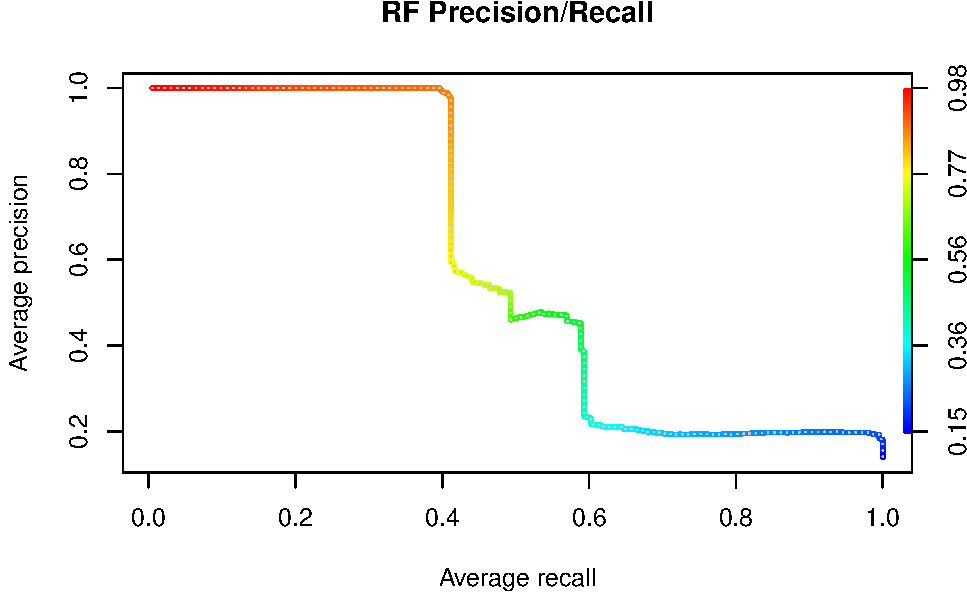
\includegraphics{gibbonR_tutorial_files/figure-latex/unnamed-chunk-13-1.pdf}

\begin{verbatim}
#> [1] 0.936898
\end{verbatim}

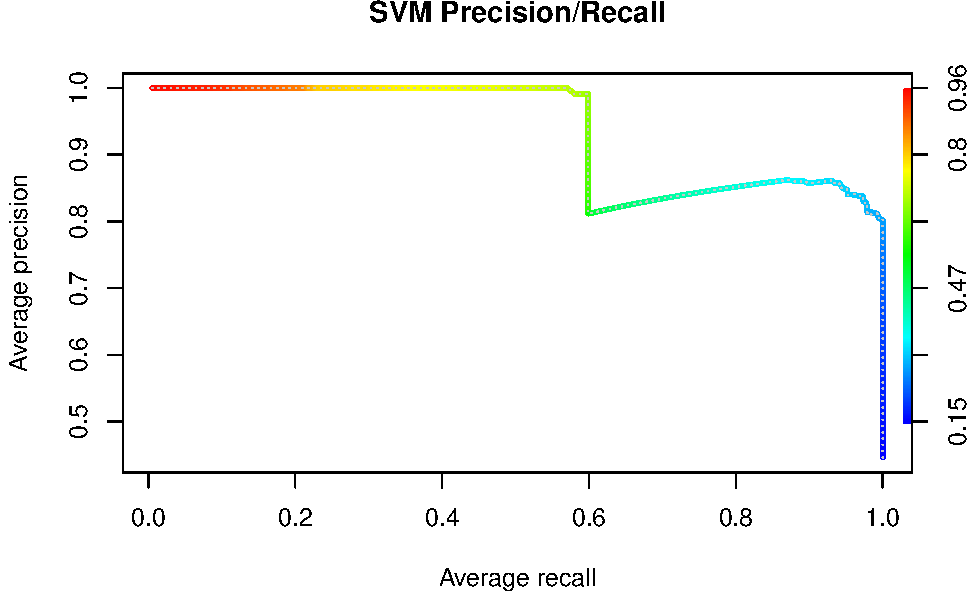
\includegraphics{gibbonR_tutorial_files/figure-latex/unnamed-chunk-13-2.pdf}

\hypertarget{part-4.-data-visualization}{%
\chapter{Part 4. Data visualization}\label{part-4.-data-visualization}}

\hypertarget{part-4a.-create-a-umap-plot-colored-by-class}{%
\section{Part 4a. Create a UMAP plot colored by class}\label{part-4a.-create-a-umap-plot-colored-by-class}}

\begin{Shaded}
\begin{Highlighting}[]
\FunctionTok{library}\NormalTok{(gibbonR)}
\FunctionTok{library}\NormalTok{(ggpubr)}
\CommentTok{\#\textgreater{} Loading required package: ggplot2}
\CommentTok{\#\textgreater{} }
\CommentTok{\#\textgreater{} Attaching package: \textquotesingle{}ggplot2\textquotesingle{}}
\CommentTok{\#\textgreater{} The following object is masked from \textquotesingle{}package:randomForest\textquotesingle{}:}
\CommentTok{\#\textgreater{} }
\CommentTok{\#\textgreater{}     margin}
\FunctionTok{UMAPBiplotAddSpectrograms}\NormalTok{(}\AttributeTok{input.dir.Focal=}\StringTok{"/Users/denaclink/Desktop/RStudio Projects/gibbonR/data/MultipleSoundClasses/"}\NormalTok{,}\AttributeTok{output.dir.Focal=}\StringTok{"/Users/denaclink/Desktop/RStudio Projects/gibbonR/data/MultipleSoundClasses/Thumbnails/"}\NormalTok{,}\AttributeTok{add.spectrograms=}\ConstantTok{TRUE}\NormalTok{,}\AttributeTok{min.freq=}\DecValTok{400}\NormalTok{,}\AttributeTok{max.freq=}\DecValTok{1600}\NormalTok{,}\AttributeTok{main=}\StringTok{"UMAP Plot"}\NormalTok{)}
\CommentTok{\#\textgreater{} [1] "Step 1 Calculating MFCCs"}
\CommentTok{\#\textgreater{} [1] "Step 2 Creating biplot"}
\CommentTok{\#\textgreater{} [1] "Step 3 Creating Spectrograms"}
\CommentTok{\#\textgreater{} [1] "/Users/denaclink/Desktop/RStudio Projects/gibbonR/data/MultipleSoundClasses/Thumbnails/ already exists"}
\CommentTok{\#\textgreater{} [1] "Step 4 Adding Spectrograms to Plot "}
\end{Highlighting}
\end{Shaded}

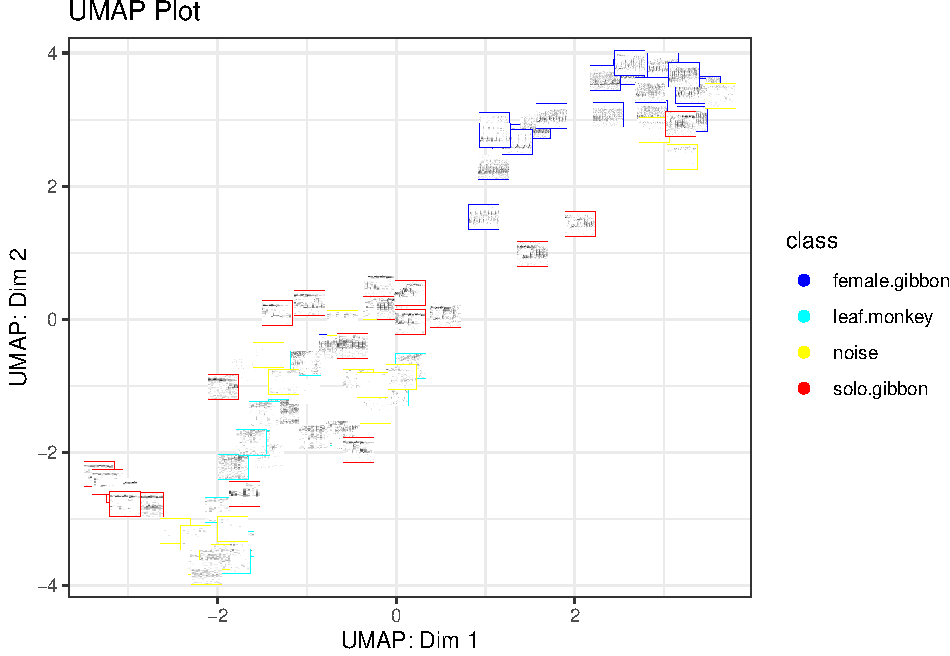
\includegraphics{gibbonR_tutorial_files/figure-latex/unnamed-chunk-14-1.pdf}
\#\# Part 4b. Create a UMAP plot colored by affinity propagation clustering

\begin{Shaded}
\begin{Highlighting}[]
\FunctionTok{library}\NormalTok{(gibbonR)}
\FunctionTok{library}\NormalTok{(ggpubr)}
\FunctionTok{library}\NormalTok{(apcluster)}
\CommentTok{\#\textgreater{} }
\CommentTok{\#\textgreater{} Attaching package: \textquotesingle{}apcluster\textquotesingle{}}
\CommentTok{\#\textgreater{} The following object is masked from \textquotesingle{}package:stats\textquotesingle{}:}
\CommentTok{\#\textgreater{} }
\CommentTok{\#\textgreater{}     heatmap}
\FunctionTok{AffinityBiplotAddSpectrograms}\NormalTok{(}\AttributeTok{input.dir.Focal=}\StringTok{"/Users/denaclink/Desktop/RStudio Projects/gibbonR/data/MultipleSoundClasses/"}\NormalTok{,}\AttributeTok{output.dir.Focal=}\StringTok{"/Users/denaclink/Desktop/RStudio Projects/gibbonR/data/MultipleSoundClasses/Thumbnails/"}\NormalTok{,}\AttributeTok{class=}\StringTok{\textquotesingle{}fixed\textquotesingle{}}\NormalTok{, }\AttributeTok{q.fixed=}\FloatTok{0.1}\NormalTok{,}\AttributeTok{add.spectrograms=}\ConstantTok{TRUE}\NormalTok{,}\AttributeTok{min.freq=}\DecValTok{400}\NormalTok{,}\AttributeTok{max.freq=}\DecValTok{1600}\NormalTok{,}\AttributeTok{main=}\StringTok{"UMAP Plot"}\NormalTok{)}
\CommentTok{\#\textgreater{} [1] "Step 1 Calculating MFCCs"}
\CommentTok{\#\textgreater{} [1] "Step 2 Computing unsupervised clustering with fixed q"}
\CommentTok{\#\textgreater{} [1] "Step 3 Creating Spectrograms "}
\CommentTok{\#\textgreater{} [1] "/Users/denaclink/Desktop/RStudio Projects/gibbonR/data/MultipleSoundClasses/Thumbnails/ already exists"}
\CommentTok{\#\textgreater{} [1] "Adding Spectrograms to Plot Step 3 of 3"}
\end{Highlighting}
\end{Shaded}

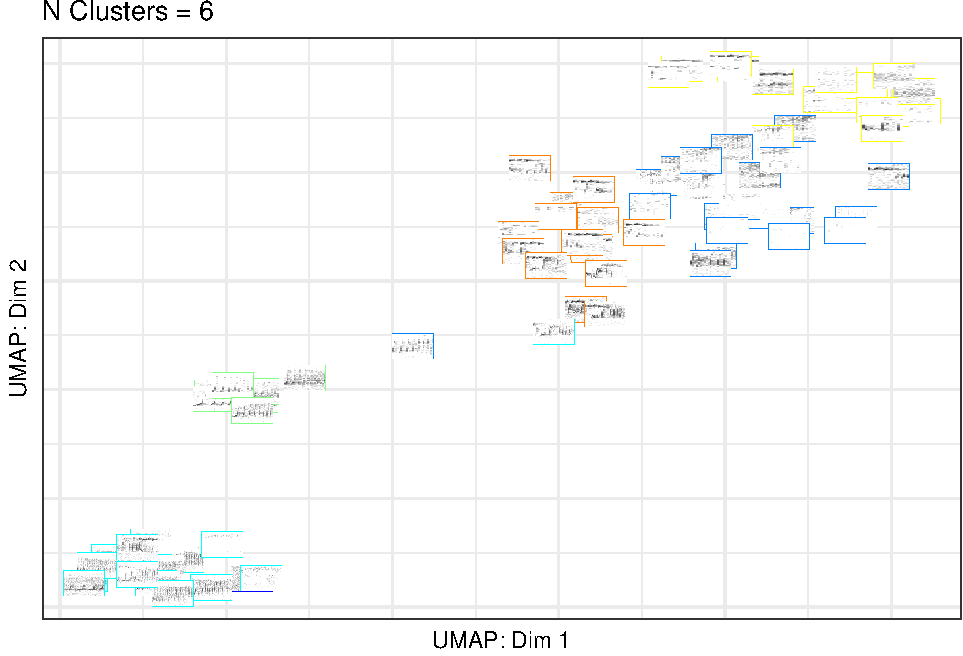
\includegraphics{gibbonR_tutorial_files/figure-latex/unnamed-chunk-15-1.pdf}

  \bibliography{book.bib,packages.bib}

\end{document}
